% ##################################################################################################################
\chapter{Yokohama: MATSim Application for Resilient Urban Design}
\label{ch:yokohama}
\hfill \textbf{Authors:} Yoshiki Yamagata, Hajime Seya, Daisuke Murakami

% ##################################################################################################################
\section{Introduction}
In Yamagata and Seya (2015) \citet[][]{}, we proposed the concept of a resilient local electricity-sharing system as a complement or alternative to a feed-in tariff (FiT) to achieve $CO_2$-neutral transportation in cities. In our proposed system, electricity generated from widely introduced solar photovoltaic panels (PVs) \ah{glossary} is stored in the cars ``not in use'' in a city. In Japan, almost half of the cars in the central Tokyo metropolitan area are used only on weekends and thus are kept parking during weekdays. These cars represent a huge new potential storage if they were replaced by \glspl{ev}, that is, they could be used as storage batteries in a V2C (Vehicle to Community) \ah{glossary} system. 

The objective of this study is to analyze the potential of \glspl{ev} as storage batteries in emergency cases. Specifically, we focus on the following three questions: 
\begin{enumerate}\styleEnumerate
\item How much of the residential demands can be filled by the electricity from PVs only, which are installed on the roofs of all detached houses in the study area in each 24\,hour? 
\item How many EVs are needed to store all surplus electricity (PV supply minus demand)?
\item How EVs driving changes the load curve, and how mass-adopted PVs can fulfil total demand? 
\end{enumerate}
To answer our second and third questions, we needed to know (a) the number of cars parking at home during each hour (that is, the time each car arrived at home after use) and (b) the amount of battery charge consumed by each driver during his/her daily trips (that is, trip duration). For this simulation, we used \gls{matsim}. In this chapter, we briefly introduce our \gls{matsim} application for a local electricity-sharing system in Yokohama city, based on Yamagata and Seya (2013) and Yamagata et al. (2014; 2015) \citet[][]{}.

% ##################################################################################################################
\section{Results}
We assume that PV was installed on the roof of each detached house in Yokohama city. Then we calculated the amount of electricity supplied during each hour throughout the whole day by employing simple intensity method. Our target period was 2008; the data we gathered are summarized in Table~\ref{tab:yokohama_tab1}. The \gls{od} trip data that we used are from the Fourth Person Trip Survey in Tokyo Metropolitan Area, which was implemented in 1998. The data are available through the People Flow Project (\url{http://pflow.csis.u-tokyo.ac.jp}) upon request (application) and include the \gls{od} trips by traffic mode, time of day, purpose, etc. for each micro district, called \emph{cho-cho-moku}. The Person Trip survey is a national survey that focuses on people's travel behavior during a given few days of each month, from October to December. Because the number of cars in Yokohama for each cho-cho-moku is unknown, the city-level value was allocated to the cho-cho-moku (areal weighting) and adjusted for the size of the population. The road-network information was taken from the National Digital Road Map Database and includes sufficient data regarding road capacity, width classification, link length, number of lanes, and travel speed to perform traffic simulations in MATSim. MATSim requires a daily ``plan file'' for each agent (car driver); we prepared these files by using the Fourth Person Trip Survey, which captured the daily movements of 722\,000 people. Because the Fourth Person Trip Survey sampled approximately 2\,\% of the population of the Tokyo metropolitan area, the plan file was replicated according to the intensity factor provided by the People Flow Project, resulting in 505\,335 agents. From the \gls{matsim} simulation, we had obtained both trip duration and arrival time of each agent. 

Considering the load curve changes due to the \glspl{ev} driving, we then asked if massively adopted PVs would be enough to satisfy the total energy demand in Yokohama. In Figure~\ref{fig:yokohama_fig1}, the solid and dashed lines represent the cumulative distribution of electricity surplus, charged to or discharged from the batteries of EVs, not in use and used only for charging the \glspl{ev} in use, during May and August (solid line, maximum; dashed line, average). The dotted line in the figure represents the scenario in which the electricity surplus was used both for charging \glspl{ev} in use and satisfying the households' typical demand. Surprisingly, in May, it was shown that the EV charged electricity surplus was far more sufficient for charging both \glspl{ev} and satisfying the households' typical electricity demand under maximal/average solar irradiance. However, in August (high demand, high PV supply), the electricity surplus was sufficient for charging \glspl{ev} but was not enough to meet the households' huge electricity demand due to the air-conditioning in evening. 
%
 %------------
\createfigure%
{Cumulative distribution of electricity surplus charged to or discharged for electricity demand (y axis denotes the cumulative distribution of electricity surplus)}%
{Cumulative distribution of electricity surplus charged to or discharged for electricity demand (y axis denotes the cumulative distribution of electricity surplus)}%
{\label{fig:yokohama_fig1}}%
{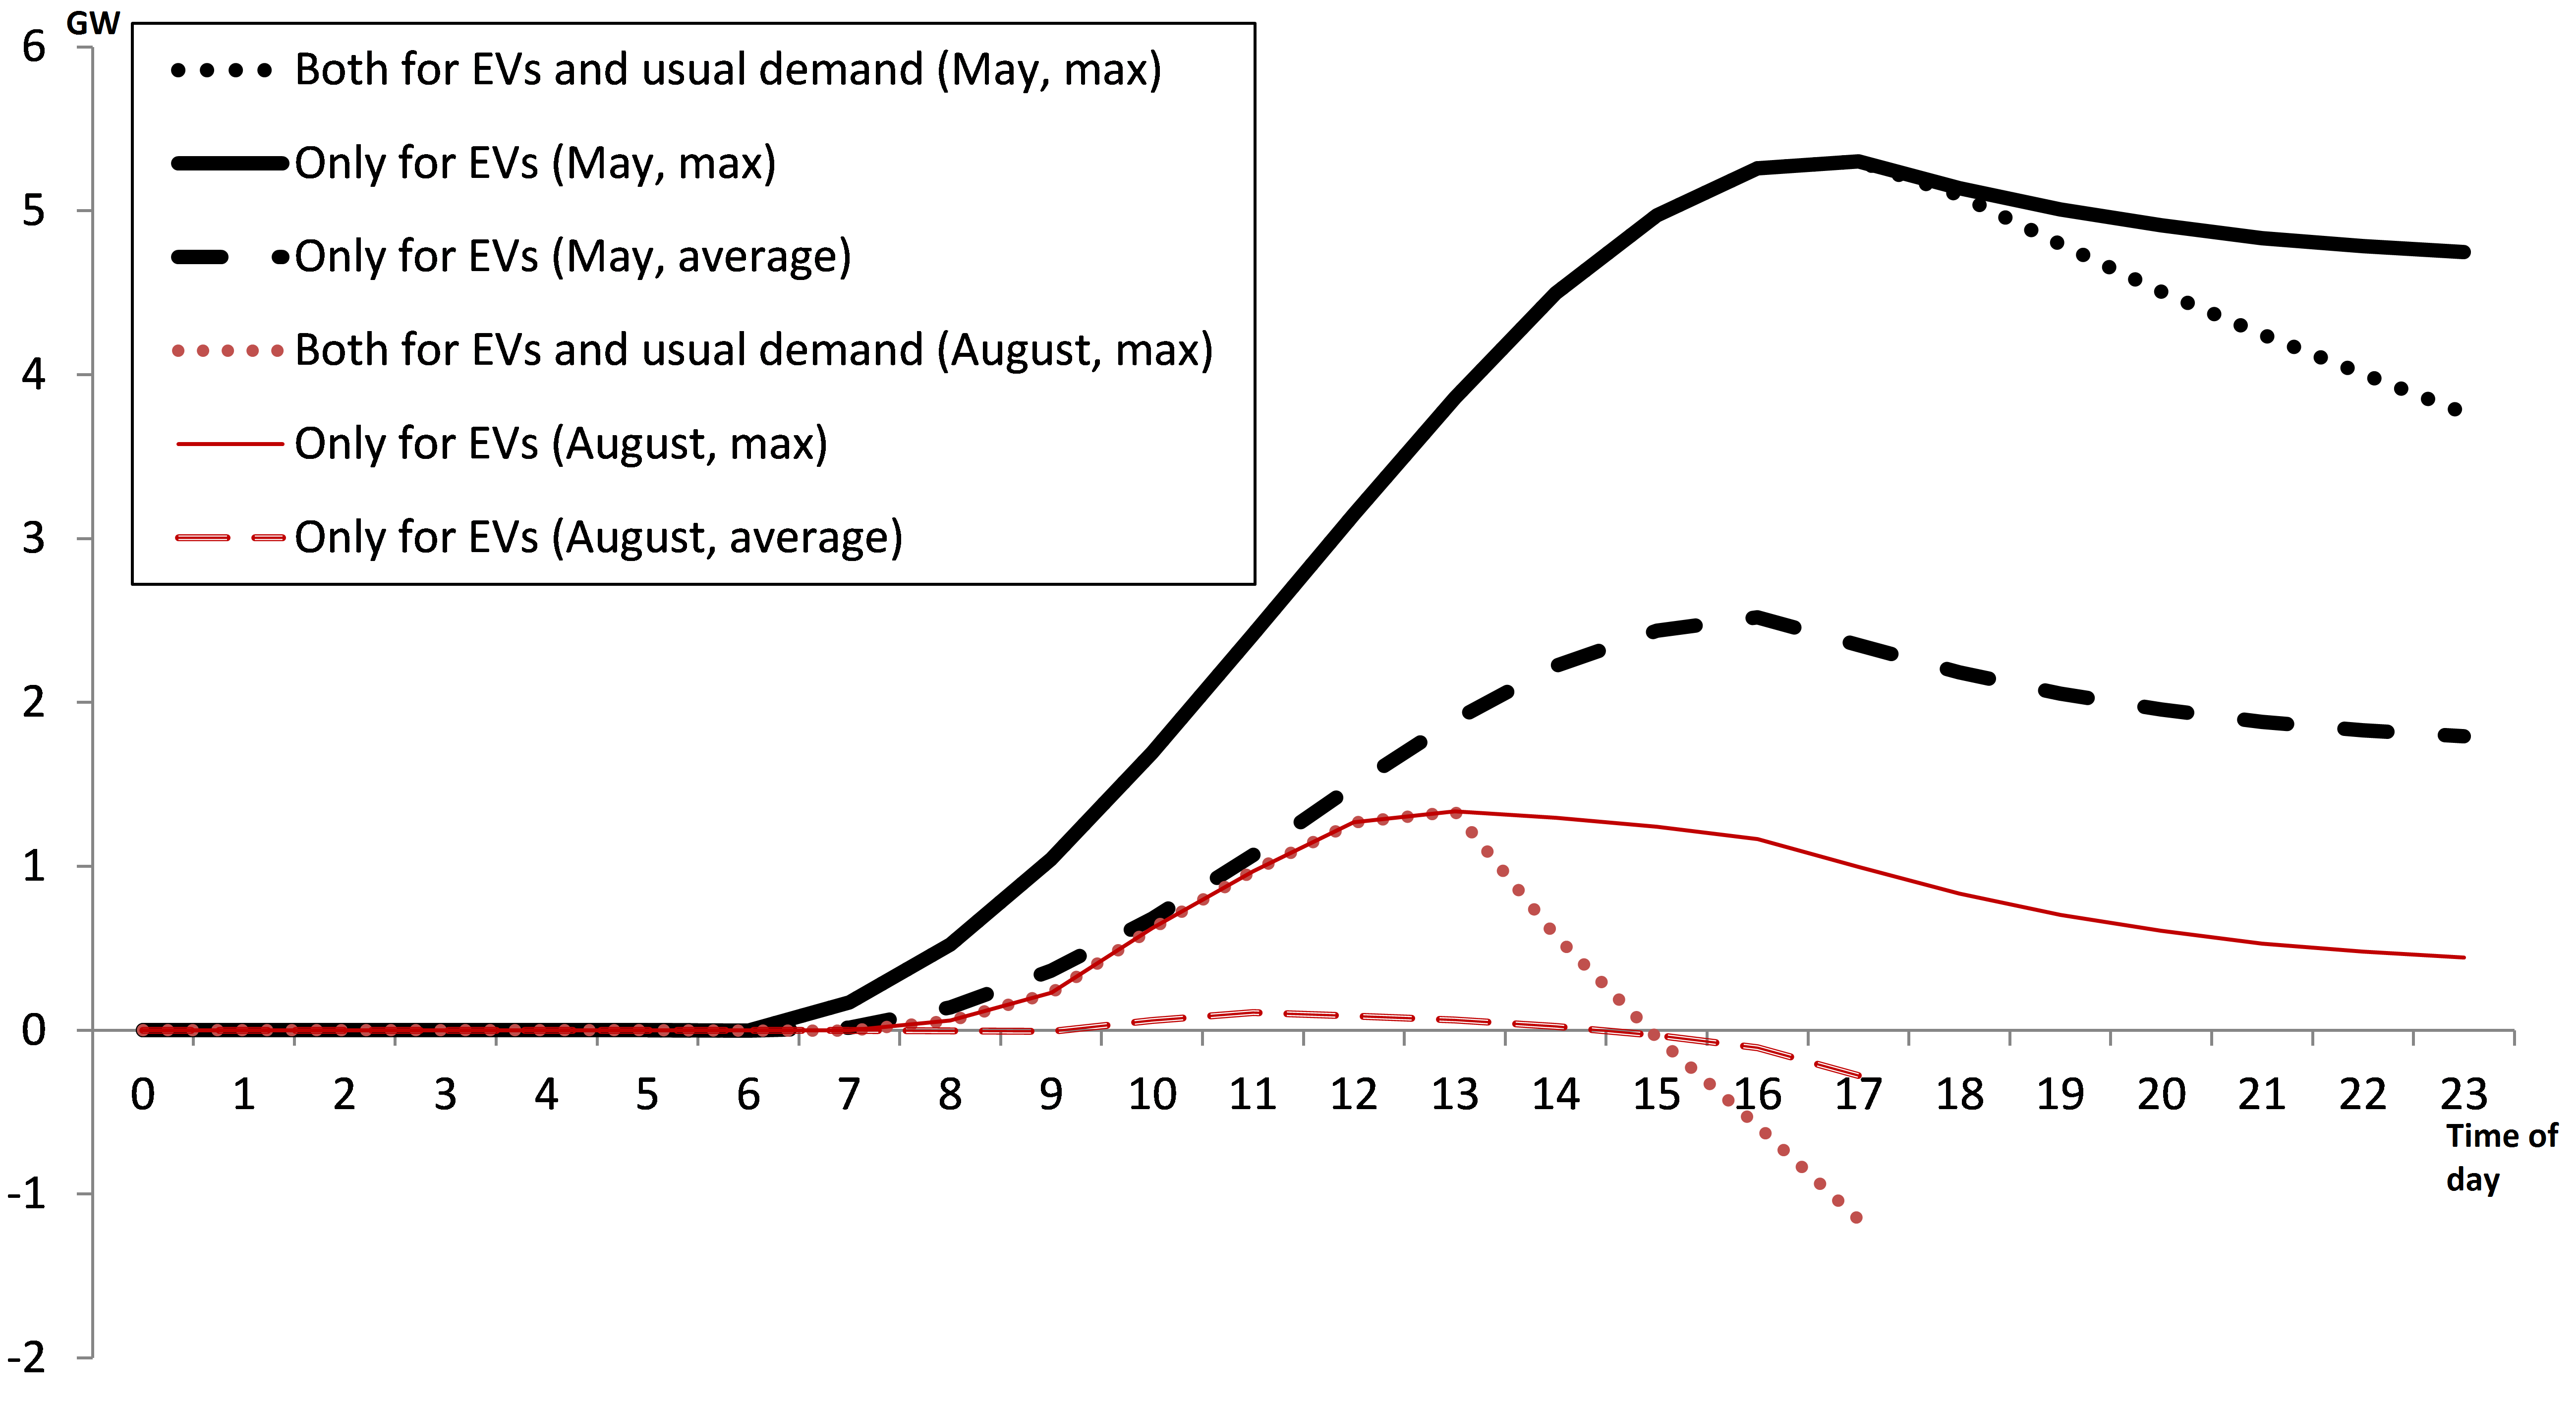
\includegraphics[width=0.99\textwidth, angle=0]{./scenarios/figures/yokohama_fig1.png}}%
{}
 %------------

To fulfill the household electricity demand, PV electricity need be stored into \glspl{ev} efficiently and locally shared. For example, if a high-affordability zone (storage capacity is greater than electricity surplus) is adjacent to a low-affordability zone (storage capacity is smaller than electricity surplus), then share of their \gls{ev} capacity increases the ratio of stored PV electricity. Because storage affordability (storage capacity minus electricity surplus) has significant regional differences (see Figure~\ref{fig:yokohama_fig2}), the clustering of the community-based local sharing need to be carefully designed. In this study, we have attempted to optimize the community clusters by several different algorithms. Firstly, the number of clusters is assumed 18 to be the same with the number of the wards in Yokohama city. Then, the cluster optimization is performed by minimizing (the sum of storage affordability in the 18\,clusters) plus $k$ (minimum circularity in these clusters), where $k$ is the weight for the circularity. The first term balances the storage capacity and the electricity surplus to increases the rate of stored PV electricity, and the second term decreases inter-point distance within each cluster, and electricity sharing (transmission) cost as well. The minimization is conducted in every month by a simulated annealing algorithm to find optimal spatially clustered communities).
%
 %------------
\createfigure%
{Storage affordability: Storage capacity minus electricity surplus in kWh/day (10\,\% of \glspl{ev} not in use being used as battery)}%
{Storage affordability: Storage capacity minus electricity surplus in kWh/day (10\,\% of \glspl{ev} not in use being used as battery)}%
{\label{fig:yokohama_fig2}}%
{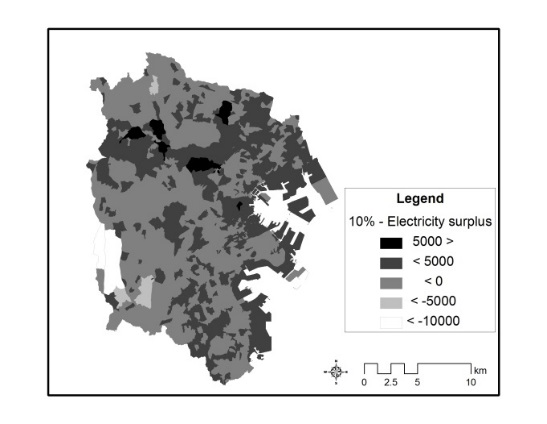
\includegraphics[width=0.99\textwidth, angle=0]{./scenarios/figures/yokohama_fig2.png}}%
{}
 %------------
%
 %------------
\createfigure%
{Monthly clustering results}%
{Monthly clustering results}%
{\label{fig:yokohama_fig3}}%
{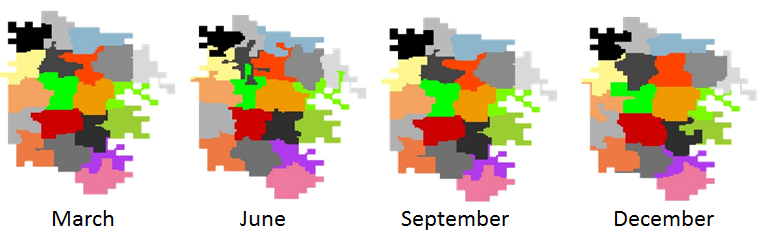
\includegraphics[width=0.99\textwidth, angle=0]{./scenarios/figures/yokohama_fig3.png}}%
{}
 %------------

Figure~\ref{fig:yokohama_fig3} shows the clustering results in four months. All clusters indicate positive storage affordability in April, May, June, July, September, and October. In other words, PV electricity covers whole household electricity demands if \gls{ev} capacities are shared with these optimized clusters.

In summary, we applied \gls{matsim} to analyze the potential of \glspl{ev} in a V2C system, and revealed that EVs can cover typical household electricity demands in some months, and the cover ratio can be increased by a community clustering for local electricity sharing. In the future study, we plan to use \gls{matsim} to simulate mobility behavior for electricity sharing community scenarios, and extend our clustering analysis utilizing the simulated behavior. Finally, development of community level mobility sharing service would be a very important topic to integrate the MATSim simulations with our land use and transportation scenarios, such as compact and dispersion scenarios (see, Yamagata et al., 2013) \citep[][]{}.

% ##################################################################################################################